\subsection{Classification: logistic regression and discriminant analysis}
\label{sec:clasificacion_tecs}

The factor scores of \cref{sec:analisis-factorial} are joined by station and
date with the categorical variables of the station-day and with the response
\texttt{excede\_anio\_5}. The scores do not have unit variance (standard
deviations of 1.14, 1.10 and 1.21 in the fitting period), so they are
rescaled with the mean and standard deviation of 2021--2024, never with those
of 2025; each odds ratio is then read per standard deviation of the factor,
and the three are comparable with one another. The categorical variables
\texttt{zona}, \texttt{tipo\_dia} and \texttt{temporada} enter as 12
indicators against the reference levels Northeast, weekday and winter. The
design matrix has 15 predictors; 16,058 rows enter the fit and 2,978 the
validation.

\subsubsection{Logistic regression}\label{sec:reg_log}

The model is fitted on 2021--2024 only. The odds ratios are reported in
\cref{tab:momios-log}; no interval for the three factors crosses 1.
Photochemical forcing has the largest effect: one additional standard
deviation multiplies the odds of exceedance by 2.78, versus 1.92 for primary
combustion. The reading is chemical: precursors are necessary, but the rate
and volume of the reactions that produce ozone depend on temperature and
radiation, so the photochemical condition weighs more than the availability
of ingredients. Ventilation is the only protective factor (0.90): wind
disperses.

\begin{table}[pos=t]
  \centering
  \caption{Odds ratios of the logistic model (\texttt{exp} of the
    coefficient) with 95\,\% interval under independence. Factors are
    interpreted per standard deviation; indicators, against their reference
    level: Northeast (zone), weekday (\texttt{tipo\_dia}) and winter
    (\texttt{temporada}). All coefficients are significant ($p<0.001$)
    except \texttt{tipo\_dia\_sabado} ($p=0.04$) and
    \texttt{tipo\_dia\_festivo} ($p=0.13$).}
  \label{tab:momios-log}
  \small
  \begin{tabular}{lrc}
    \toprule
    Variable & Odds ratio & 95\,\% CI \\
    \midrule
    Primary combustion      & 1.92 & [1.82, 2.02] \\
    Ventilation             & 0.90 & [0.86, 0.95] \\
    Photochemical forcing   & 2.78 & [2.62, 2.94] \\
    \midrule
    \texttt{zona\_Centro}    & 2.74 & [2.32, 3.22] \\
    \texttt{zona\_Noroeste}  & 3.84 & [3.32, 4.43] \\
    \texttt{zona\_Norte}     & 1.76 & [1.50, 2.06] \\
    \texttt{zona\_Sur}       & 2.90 & [2.44, 3.44] \\
    \texttt{zona\_Sureste}   & 1.82 & [1.59, 2.09] \\
    \texttt{zona\_Suroeste}  & 3.48 & [3.02, 4.01] \\
    \midrule
    \texttt{tipo\_dia\_sabado}  & 1.13 & [1.01, 1.27] \\
    \texttt{tipo\_dia\_domingo} & 1.43 & [1.27, 1.62] \\
    \texttt{tipo\_dia\_festivo} & 1.17 & [0.95, 1.44] \\
    \midrule
    \texttt{temporada\_primavera} & 3.54 & [3.08, 4.08] \\
    \texttt{temporada\_verano}    & 1.54 & [1.31, 1.83] \\
    \texttt{temporada\_otono}     & 3.04 & [2.66, 3.49] \\
    \bottomrule
  \end{tabular}
\end{table}

The zones with the highest odds are Northwest (3.84) and Southwest (3.48):
for the same meteorology and calendar, the west of the city almost
quadruples the odds of the Northeast, the spatial ordering anticipated in
\cref{sec:contexto-estaciones}. Spring (3.54) and autumn (3.04) triple the
odds of winter, which, with lower temperature and radiation, slows the
photochemical reactions even when precursors are present; summer stays at
1.54. The working calendar has little influence: only Sunday (1.43) has a
clear effect.

\paragraph{Standard errors under dependence.} The 15 stations on the same day
share the weather, and consecutive days resemble each other, so standard
errors under independence are optimistic. They are corrected with the
sandwich estimator clustered by day (1,460 clusters): they inflate by
1.5 to 2.5 times, more for the calendar indicators, which are constant
within a day, and not at all for the zone indicators, which vary within it.
The corrected intervals of the three factors are almost twice as wide and
still do not cross 1 (\cref{fig:momios-corregido}): ventilation
$[0.84, 0.97]$, photochemical forcing $[2.48, 3.10]$. The only term that
loses significance at 5\,\% is Saturday. Clustering also by station is not
reliable with 15 clusters, but it makes clear that the six zone contrasts
rest on 15 units, not on 16,058 rows.

\begin{figure}[pos=t]
  \centering
  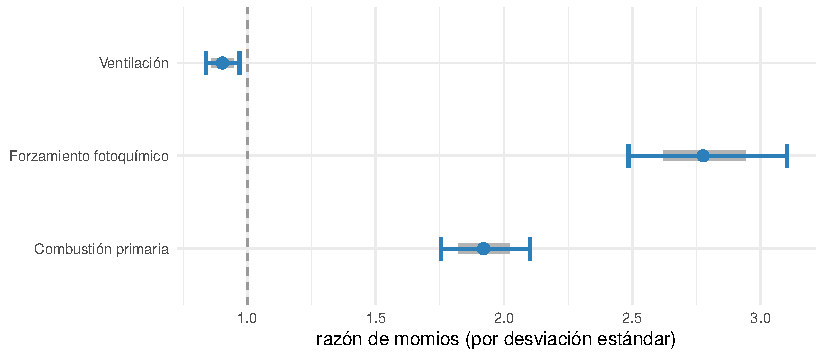
\includegraphics[width=\linewidth]{momios_ic_corregido.pdf}
  \caption{Odds ratios of the factors with 95\,\% intervals under
    independence (gray) and clustered by day (color). The corrected
    intervals are wider and none crosses 1.}
  \label{fig:momios-corregido}
\end{figure}

\paragraph{Evaluation and validation.} Evaluation is performed on 2025, not
seen during fitting, with AUC, sensitivity and specificity; accuracy is
discarded because the base exceedance rate in validation is 43.97\,\%. The
model reaches an AUC of 0.850 (\cref{fig:roc-modelos}), above the
performance threshold of 0.75. The classification threshold is chosen by
Youden's index on the fitting data and equals 0.282; at that threshold
sensitivity is 0.698 and specificity 0.853 (left panel of
\cref{fig:matrices}). A threshold of 0.5 illustrates why accuracy is not a
suitable criterion: specificity rises to 0.964, but sensitivity falls to
0.326, that is, the model misses two of every three actual exceedances.

\subsubsection{Linear discriminant analysis}\label{sec:lda}

The second technique is fitted on the same design matrix, the same response
and the same partition. The contrast is deliberate: the discriminant assumes
multivariate normality within each class and homoscedasticity between
classes, assumptions the logistic model does not require.

\paragraph{Checking assumptions.} The factor scores are linear combinations
of predictors with $|\text{skewness}|<0.5$ after Box-Cox. On the training
scores split by class, the six skewness coefficients lie between $-0.091$
and 0.489, so the normal approximation holds. Homoscedasticity does not: Box's
M test, which with more than 15,000 observations rejects arbitrarily small
differences, is not applied; instead, the class covariance matrices are
compared directly. Exceedance days are less dispersed than non-exceedance
days on all three factors, with standard deviation ratios of 0.894, 0.888
and 0.742, and the generalized variance drops from 1.081 to 0.346; the
discrepancy is concentrated on the photochemical axis. A second departure
affects the 12 binary indicators, which are not normal under any
transformation. Linear discriminant analysis tolerates both departures in
practice, and that tolerance is verified empirically in
\cref{sec:comparacion}.

\paragraph{Fit and evaluation.} The prior probabilities are set to the
proportions observed in the fitting period (0.706 and 0.294) because the base
rate is information about the problem. With two classes there is a single
discriminant function, and the order and sign of its coefficients reproduce
those of \cref{tab:momios-log}: photochemical forcing (0.795) dominates
primary combustion (0.506), ventilation works against exceedance ($-0.109$),
Northwest and Southwest are the highest-risk zones, and spring (1.054) and
autumn (0.772) weigh more than summer (0.176). The coefficients give the
direction of maximum separation between classes; they are not odds ratios.
Evaluation uses the posterior probability of exceedance as a continuous
score, so that the ROC curve is comparable with the logistic one. The
discriminant reaches an AUC of 0.846; at Youden's threshold (0.249)
sensitivity is 0.758 and specificity 0.788 (right panel of
\cref{fig:matrices}).

\subsubsection{Comparison of the two models}\label{sec:comparacion}

The two techniques are practically equivalent on these data: the AUCs differ
by three thousandths (0.850 versus 0.846), the scores correlate at 0.996, and
the classifications agree on 93.8\,\% of the validation station-days.
DeLong's test for correlated ROC curves does detect the difference
($Z=3.75$, $p=0.0002$, 95\,\% CI $[0.002, 0.005]$): with 2,927 observations
it has power for three thousandths, a statistically real difference with no
practical consequence. Where they do differ is in the distribution of errors
at Youden's threshold: the discriminant detects more exceedances
(sensitivity 0.758 versus 0.698) at the cost of more false alarms
(specificity 0.788 versus 0.853).

\begin{figure}[pos=t]
  \centering
  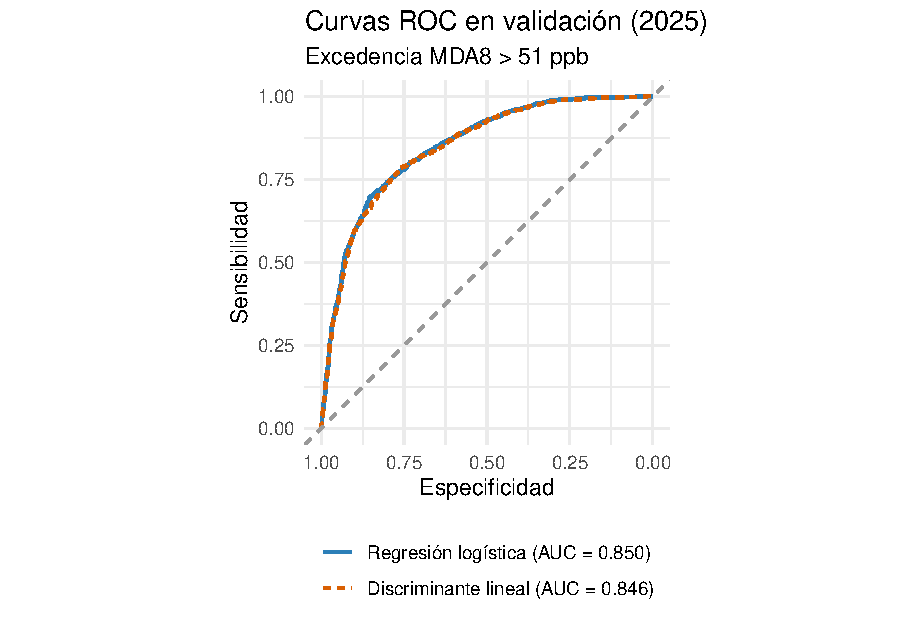
\includegraphics[width=\linewidth]{roc_modelos.pdf}
  \caption{ROC curves of both models on the validation partition (2025). The
    two curves overlap; the discriminant is drawn dotted.}
  \label{fig:roc-modelos}
\end{figure}

\begin{figure}[pos=t]
  \centering
  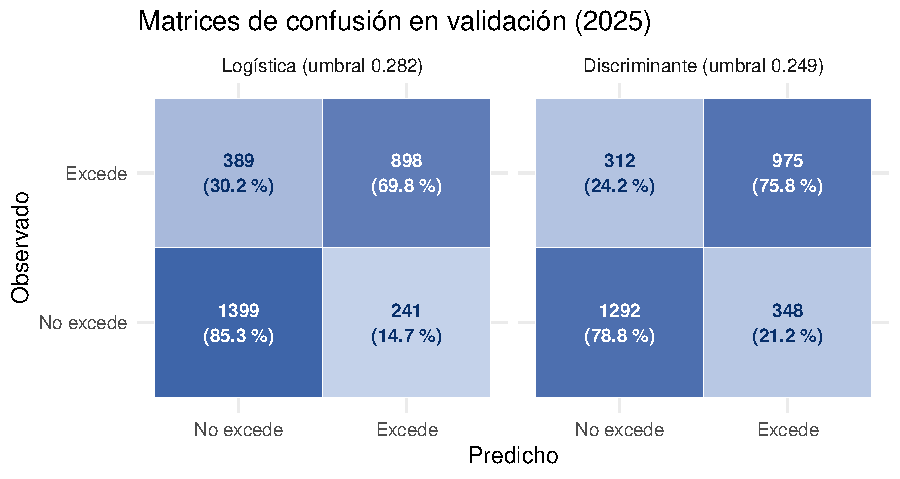
\includegraphics[width=\linewidth]{matriz_confusion.pdf}
  \caption{Confusion matrices in validation, each model at its own Youden
    threshold. Percentages are row proportions (observed class).}
  \label{fig:matrices}
\end{figure}

This agreement is the relevant result: the heteroscedasticity documented in
\cref{sec:lda} is real and still does not alter performance, so the decision
boundary drawn by both is the same, and the interpretation of the odds
ratios does not depend on the normality assumption that the discriminant
requires and the logistic model does not. As an additional contrast, the
logistic model on the PCA scores reaches an AUC of 0.848 (DeLong $p=0.44$
versus 0.850): the factors lose no discriminating power and gain
interpretability.

\paragraph{Error rate correction.} The apparent resubstitution error (0.229
for the logistic model, 0.230 for the discriminant) barely changes with
10-fold cross-validation by whole days (0.231 and 0.232) or with
Lachenbruch's method (0.231): with 16 parameters on 15,704 observations the
optimism is of order $p/n$, and neither classifier overfits. What
cross-validation does reveal is the year effect: within 2021--2024 the
out-of-sample AUC is 0.80, not 0.85. By year, each predicted by a model that
did not see it, 2021--2023 stay at 0.76--0.77, 2024 rises to 0.84 and 2025
to 0.85. The expected performance in an arbitrary year is 0.80; the 0.85
corresponds to the two high-ozone years.

\subsubsection{Limitations}\label{sec:limitaciones-clasificacion}

\textbf{Autocorrelation.} The 18,631 station-day rows of fitting and
validation are not independent: the effective $n$ is closer to the 1,826
distinct days. The correlation between stations within the same day averages
0.53 for the response and reaches 0.85 for the photochemical factor; the
day-to-day autocorrelation of the response within each station is 0.49.
Standard errors were corrected for day clustering and the conclusions hold;
what cannot be properly corrected is the station dimension. The AUC is not
affected, because it is computed on unseen observations.

\textbf{Absence of volatile organic compounds.} The axes are described as
consistent with primary combustion, ventilation or photochemical forcing,
never as an attribution of a NOx--VOC regime. An odds ratio of 2.78 says that
days with more photochemical forcing have higher odds of exceedance; it does
not say which precursor limits ozone formation, a question that cannot be
answered with these data.

\textbf{Explanatory scope.} The predictors are from the same day as the
response: the models describe which conditions accompany an exceedance and
do not anticipate the next day's ozone.

\textbf{Validation in an atypical year.} 2025 has 44\,\% exceedance versus
29\,\% in the fitting period. The AUC dampens the base-rate bias, but
sensitivity and specificity are read on a year with more exceedance-prone
days than the series average.
